\section{Introduction}
\begin{figure}
\centering
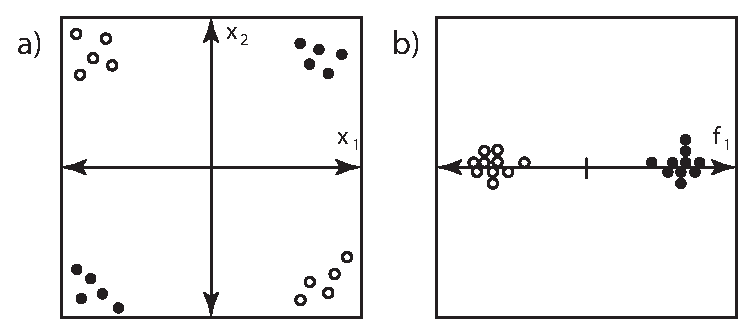
\includegraphics[height=2.7cm]{figs/xor.eps}
\caption{{\bf a)} A variation of the exclusive-or problem, named for the XOR logic table it resembles. It has be re-centered on the origin. The challenge is to separate the data points into their respective classes. It clearly cannot be achieved by a linear separation boundary. {\bf b)} The same problem with each data point expressed in a feature space with $f_1 = x_1 \times x_2$. Once transformed into this feature space, linear separation becomes straightforward.}
\label{xor}
\end{figure}

\subsection{Related work}
construction approaches, and the winners are described in the same volume as the introduction~\cite[e.g.]{torkkola03}.

\newcommand{\colwid}{6.0cm}
\newcommand{\algtab}{\hspace{0.6cm}}

\begin{table}[!t]
\centering
\begin{tabular*}{\colwid{}}{l l}
&\rule[0mm]{\colwid{}}{0.3mm}\\
&{\bf Algorithm 1}  \textsc{Feature Creator}\\
&\rule[1.0mm]{\colwid{}}{0.3mm}\\
&{\bf Input:} {\it observation} vector\\
&{\bf Output:} {\it feature\_activity} vector\\
& \\
{\scriptsize 1:}& form {\it input} vector by concatenating {\it observation} \\
&\algtab and previous {\it feature\_activity} \\
{\scriptsize 2:}& update estimate of {\it correlation} between {\it inputs}  \\
{\scriptsize 3:}& {\bf if}  \textsc{max}({\it correlation}) $> C_1$ {\bf then} \\
{\scriptsize 4:}&\algtab add the two {\it input} elements achieving the \\
&\algtab \algtab maximum {\it correlation} to the new {\it group}\\
{\scriptsize 5:}&\algtab {\bf while}  \textsc{not}({\it stop\_condition\_met}) {\bf do}\\
{\scriptsize 6:}&\algtab \algtab find {\it mean\_correlation} between each \\
&\algtab \algtab \algtab remaining {\it input} and {\it group} members\\
{\scriptsize 7:}&\algtab \algtab {\bf if} \textsc{max}({\it mean\_correlation})$ > C_2$ and \\
&\algtab \algtab \algtab {\it group} size $< C_3$ {\bf then}  \\
{\scriptsize 8:}&\algtab \algtab \algtab add the {\it input} element to the {\it group}  \\
{\scriptsize 9:}&\algtab \algtab {\bf else} {\it stop\_condition\_met}  \\
{\scriptsize 10:}& {\bf for} each {\it group} {\bf do} \\
{\scriptsize 11:}&\algtab {\bf if} \textsc{min} (\textsc{distance} ({\it input, features}))$ > C_4$ {\bf then} \\
{\scriptsize 12:}&\algtab \algtab  add normalized {\it input} to set of {\it feature}s\\
{\scriptsize 13:}&\algtab {\bf for} each {\it feature} {\bf do} \\
{\scriptsize 14:}&\algtab \algtab {\it feature\_vote} = {\it feature} $\cdot$ {\it input} \\
{\scriptsize 15:}&\algtab {\it feature\_activity} = \textsc{wta}({\it feature\_vote})\\
&\rule[2.0mm]{\colwid{}}{0.3mm}\\
\label{alg1}
\end{tabular*}
\end{table}
